\chapter{Conclusions and Outlook}
\label{ch:conclusions}

The performance of a single four-detector \hisparc station has been investigated
using Monte Carlo simulation techniques. The energy threshold for the detection of EAS is
$\sim \SI{1}{\peta\electronvolt}$. Since the energy spectrum of cosmic rays follows a
power law with a spectral index $\gamma$ approximately equal to 2.7, most
of the observed EAS had a primary energy near the detection threshold.
A library of simulated unthinned \SI{1}{\peta\electronvolt} proton showers has
been compiled for a series of zenith angles. Using this library, the detection
performance of the station has been investigated. A \SI{1}{\peta\electronvolt}
proton shower with a zenith angle of \SI{22.5}{\degree} has a
\SI{70}{\percent} probability to be observed at a core distance of
\SI{20}{\meter}. At \SI{40}{\meter}, this probability is reduced to
\SI{30}{\percent}.

With the set of simulated showers the direction sensitivity has been analyzed.
The uncertainty in the directions have been studied and compared to calculations
which were developed for this purpose.
The reconstruction of the shower direction becomes more accurate for higher
particle multiplicities in the detectors. To understand this behavior
quantitatively, the arrival times of particles have been analyzed with the
purpose of investigating the shower front structure.
The arrival time distribution has been determined from shower data and is highly
asymmetrical. It can not be approximated by a normal distribution. Averaging
over many showers, a model for the shower front structure has been developed.
This has enabled the explanation of the uncertainties as a function of particle
multiplicity. When requiring a minimum of two particles in each corner detector
($N_\mathrm{\mip} \geq 2$), as opposed to only requiring one, the accuracy of
the reconstructed shower direction is significantly improved
(\figref{fig:results-sim-mip}).

The precision of the direction determination of EAS has been investigated as a
function of zenith angle, station size and the digitization frequency. For the
design of the station, a nominal detector distance of \SI{10}{\meter} and an ADC
sampling time of \SI{2.5}{\nano\second} were an excellent choice. The arrival
time of the shower front, as measured by the detectors, has an uncertainty of
only \SI{1.8}{\nano\second}. For simulated \SI{1}{\peta\electronvolt} proton
showers with a zenith angle of \SI{22.5}{\degree}, and $N_\mathrm{MIP} \geq 2$,
the uncertainty in the shower direction has been predicted to be $\sigma_\theta
= \SI{4.3}{\degree}$ and $\sigma_\phi = \SI{11}{\degree}$.
However, the physical observable of interest is the angular distance between the
reconstructed and the simulated direction of the shower.
For small zenith angles, all possible directions on the celestial sphere are
close together. A small uncertainty in the direction can thus result in a large
uncertainty of the azimuthal angle. For two vectors which only differ in their
azimuthal angles, $\Delta\phi = \phi_1 - \phi_2$, the angular distance is given
by \eqref{eq:angular-distance}. The angular distance between two directions
separated by $\Delta\phi = \SI{11}{\degree}$ and $\Delta\theta =
\SI{4.3}{\degree}$, for $\theta = \SI{22.5}{\degree}$, is only
\SI{5.9}{\degree}, which is beyond expectations.

The performance of a single station has been analyzed by integrating the station
into the \kascade array. The \kascade experiment provided a trigger for the
station and a dataset of fully reconstructed EAS.
The detector efficiency has been verified by studying the detector response for
a series of particle densities. The response has been described by Poisson
probabilities, and the efficiency has been found to be close to
\SI{100}{\percent} (\figref{fig:detection-efficiency}). The shower front
structure has been investigated and compared to the model
developed using the simulations.

Taking an as yet unexplained experimental uncertainty of \SI{1.6}{\nano\second}
into account, the data from simulations (\chref{ch:reconstruction}) closely
match the data from a single four-detector \hisparc station (\chref{ch:kascade})
and identical conclusions hold for both analyses. The uncertainties have been
described and are well understood as a function of particle multiplicity, core
distance and zenith angle, in both the simulation and the experiment.
The total uncertainty in the measurement has been estimated to be
\begin{equation}
\begin{split}
\sigma_t &= \sqrt{\sigma_{t,\, \mathrm{front}}^2 + \sigma_{t,\,
\mathrm{transport}}^2 + \sigma_{t,\, \mathrm{sampling}}^2 + \sigma_{t,\,
\mathrm{other}}^2} \\[5pt]
&= \sqrt{1.4^2 + 1.2^2 + \frac{2.5^2}{12} + 1.6^2} = \SI{2.4}{\nano\second}.
\end{split}
\end{equation}

For a \SI{1}{\peta\electronvolt} shower with a zenith angle of $\theta =
\SI{22.5}{\degree}$, and $N_\mathrm{\mip} \geq 2$, the resulting accuracy in the
direction of EAS has been found to be $\sigma_\theta = \SI{6.1}{\degree}$ and
$\sigma_\phi = \SI{15.9}{\degree}$. The direction of a
\SI{1}{\peta\electronvolt} shower reconstructed by \kascade is accurate to less
than \SI{0.3}{\degree} \cite{Antoni:2003gd}.
The angular distance between the direction determined by the \hisparc station
and the direction observed by \kascade, is less than \SI{8.6}{\degree} for
\SI{66}{\percent} of the reconstructed events at $\theta \approx
\SI{22.5}{\degree}$.
The uncertainties in the reconstruction must be viewed in light of the size and
cost of a single station.
A single station has an active detector surface of only \SI{2}{\square\meter}
and covers an area of \SI{43}{\square\meter}. Its cost is approximately
\EUR{10000}.

The reconstruction of shower direction has been performed with a subcluster of
three stations in the Amsterdam Science Park Array, which resembles an
equilateral triangle with sides ranging from \SIrange{122}{151}{\meter}.
First, the performance of the individual stations has been studied. The observed
cosmic ray arrival directions are indeed isotropically distributed. The zenith
angle distribution peaks around \SI{20}{\degree}.
The directions could not be compared to an external reference (simulated
direction, or the direction as provided for a single station in \kascade).
For a single shower, the reconstructed directions obtained by the individual stations agree within an
accuracy which is consistent with the calculations used in
\chtworef{ch:reconstruction}{ch:kascade}. Systematic discrepancies are absent. The
accuracy of the shower direction determined by a single station has been
verified, and it is used as a reference for the (sub)cluster.

For EAS which have been reconstructed by the subcluster and by a single station
simultaneously, the directions agree. Moreover, the uncertainties are well
described by the calculations (\figref{fig:sp-results-uncertainties}). This is a
critical observation since this demonstrates that the calculations for the
uncertainties in the direction of EAS describe the data within a timing
uncertainty of \SI{5.5}{\nano\second} (\SI{66}{\percent} of events) in the
cluster.
These calculations can then be used to estimate the precision of the shower
direction observed by the subcluster of 501, 503 and 506. The accuracy is
estimated to be $\sigma_\phi = \SI{2.7}{\degree}$ and $\sigma_\theta =
\SI{1.1}{\degree}$ at $\theta = \SI{22.5}{\degree}$. Expressed as an angular
distance, the precision then becomes \SI{1.5}{\degree}.


\section{Outlook: Towards Energy Determination of EAS}

The reconstruction of the size of an EAS is necessary to determine the
energy of the primary particle.  This can be achieved by measuring the lateral
distribution of the shower particles.  Then, a theoretical distribution of the
lateral density can be fitted to the experimentally observed distribution. The
fit parameters are the core position and the shower size. The latter can be
used to estimate the primary energy. In this section, we will give a description
of the procedure to determine the size of an EAS.

There are several lateral distribution functions given in the literature.
Some are theoretically derived or motivated, others are empirical equations
describing the experimentally observed lateral densities.  The LDF originally
used by the \kascade experiment is the Nishimura-Kamata-Greisen (NKG) function, given by
\cite{latpaper:2005}:
\begin{equation}
\label{eq:nkg}
\rho(r) = N_e\, c(s) \left(\frac{r}{R_0}\right)^{s - 2} \left(1 +
\frac{r}{R_0}\right)^{s - 4.5},
\end{equation}
with $\rho(r)$ the particle density as a function of the core distance, $N_e$
the number of electrons in the shower, $R_0$ the Molière radius, $s$ the
shower age parameter, and $c(s)$ given by:
\begin{equation}
c(s) = \frac{\Gamma(4.5 - s)}{2\pi r_0^2\, \Gamma(s)\,\Gamma(4.5 - 2s)}.
\end{equation}
This theoretically motivated function did not describe the \kascade data
accurately.  By redefining several parameters, the data are better explained.
This is achieved by writing:
\begin{equation}
\label{eq:ldf}
\rho(r) = N_e\, \tilde{c}(s) \left(\frac{r}{R_0}\right)^{s - \alpha} \left(1 +
\frac{r}{R_0}\right)^{s - \beta},
\end{equation}
with $\alpha$ and
$\beta$ free parameters. Then, $\tilde{c}(s)$ is defined by:
\begin{equation}
\tilde{c}(s) = \frac{\Gamma(\beta - s)}{2\pi r_0^2\, \Gamma(s - \alpha + 2)\,
\Gamma(\alpha + \beta - 2s - 2)}.
\end{equation}
The best fit to \kascade data is obtained with $\alpha = 1.5$, $\beta = 3.6$ and
$R_0 = 40$.

The parameter $s$ is now interpreted as a \emph{shape parameter} and does not
vary significantly for most observed EAS. By fixing $s$ the number of degrees of
freedom are reduced.  A fit of \eqref{eq:ldf} to lateral densities observed
in the simulation of \SI{1}{\peta\electronvolt} proton-induced
vertical showers results in a \emph{shower size} $\lg N_e = 4.8$ and $s =
\num{0.94}$. \eqref{eq:ldf} can be written as
\begin{equation}
\rho(r) = N_e\, \tilde{c}(s) R(r),
\end{equation}
with
\begin{equation}
R(r) = \left(\frac{r}{R_0}\right)^{s - \alpha} \left(1 +
\frac{r}{R_0}\right)^{s - \beta}.
\end{equation}

Several independent measurements of the particle density are required to
determine the values of the remaining parameters, i.e. the shower size $N_e$ and
the shower core position $x, y$. These measurements are obtained if an EAS is
observed by multiple \hisparc stations. The determination of the
parameters can be simplified by considering \emph{relative}
particle densities:
\begin{equation}
\tilde{\rho_i}(r_i) = \frac{\rho_i(r_i)}{\rho_0(r_0)} = \frac{R(r_i)}{R(r_0)},
\end{equation}
with the subscripts denoting the station index. Here, station 0 is
chosen as a reference to which all other stations ($i$) will be compared.
Defining the $\chi^2$-distribution by
\begin{equation}
\chi^2 = \sum_{i\neq 0}\left(\frac{\tilde\rho_{i,\,\mathrm{ldf}} -
\tilde\rho_{i,\,\mathrm{obs}}}{\sigma_i}\right)^2,
\end{equation}
a minimization procedure provides values for the core position. For low
particle densities, the uncertainties in the particle densities are
not normally distributed. Therefore, the $\chi^2$-distribution can only be
used as an approximation. In \figref{fig:core-one}, contour plots of the
$\chi^2$-distribution are presented.  The detectors in this simulation have
precise knowledge of the particle densities in the shower. The algorithm
correctly finds the global minimum, denoted by the blue circle. The positions of the
detectors are depicted by the red circles, with the size of the circle
proportional to the observed particle density. The figure on the right shows a
geometric interpretation of the $\chi^2$-distribution by multiplying, instead of
summing, the terms. Using this interpretation, analytical approximations can be
attempted \cite{Montanus:2010}.
\begin{figure}
\centering
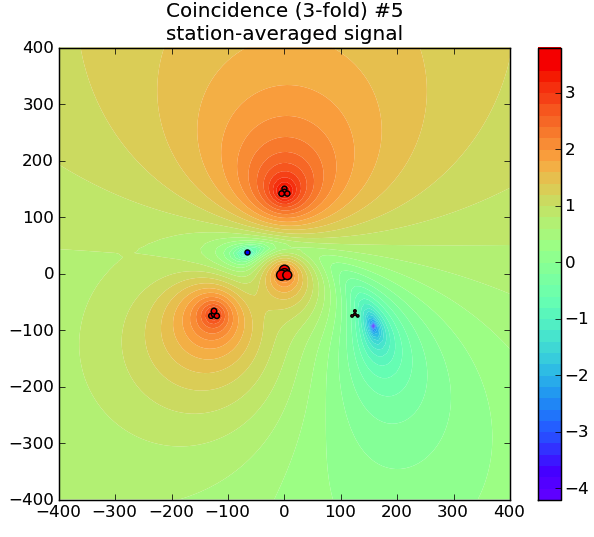
\includegraphics[width=.48\linewidth]{raw-plots/plot_core_chi_sq.png}
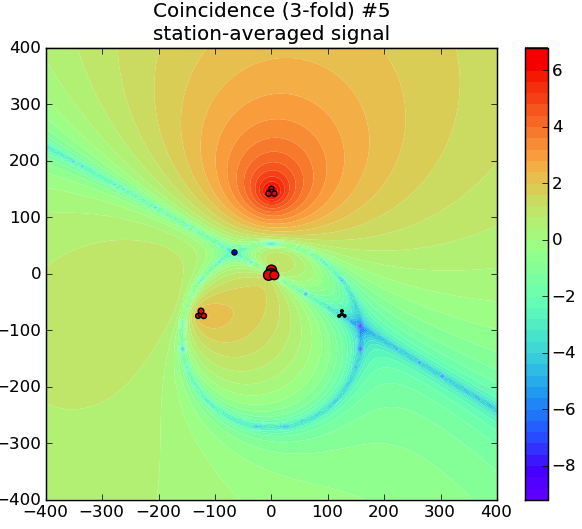
\includegraphics[width=.48\linewidth]{raw-plots/plot_core_chi_sq_alt.png}
\caption{Contour plot of the $\chi^2$-distribution (left) used in the
reconstruction of the core position. The detectors in this simulation have
precise knowledge of the particle densities in the shower. The algorithm
correctly finds the global minimum, denoted by the blue circle. The
positions of the detectors are depicted by the red circles, with the size
of the circle proportional to the observed particle density. Right: the
terms in the $\chi^2$-distribution are multiplied instead of summed,
resulting in a geometric interpretation of the solution, located at the
intersection of the two circles. One circle is very large, resulting in a
nearly straight line in the plot.}
\label{fig:core-one}
\end{figure}

\figref{fig:core-two} shows simulated and reconstructed shower core positions
for a \SI{1}{\peta\electronvolt} vertical proton.  The detectors in this
simulation have precise knowledge of the particle densities in the shower.
The reconstructed core position is, in general, very close to the simulated
position.
\begin{figure}
\centering
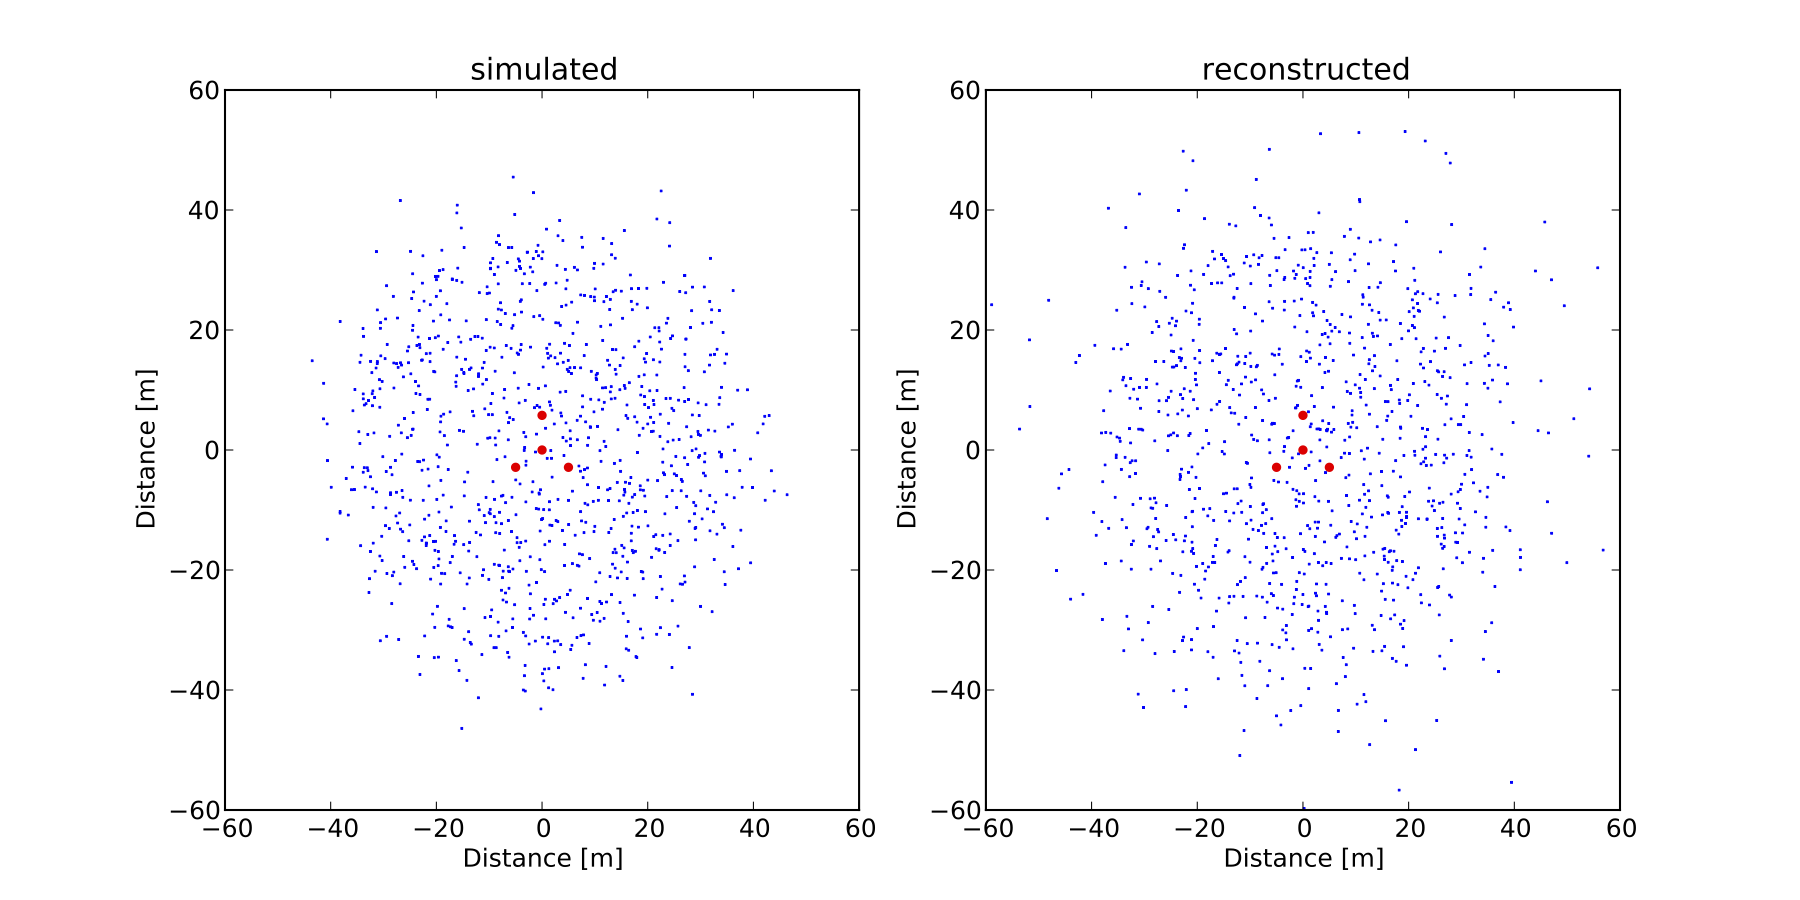
\includegraphics[width=.8\linewidth]{raw-plots/COR-plot_scatter_reconstructed_core-EXACT.png}
\caption{Simulated (left) and reconstructed (right) shower core positions
for a \SI{1}{\peta\electronvolt} vertical proton.  The detectors in this
simulation have exact knowledge about the particle densities in the
shower.  The reconstructed core positions are very close (to machine
precision) to the simulated positions, proving that the algorithm works.}
\label{fig:core-two}
\end{figure}
In \figref{fig:core-twob} the detector signals have
been included using the simulations discussed in \chref{ch:reconstruction}.
The detectors no longer have knowledge of the particle densities in the shower
(e.g. \SI{1.3}{\per\square\meter}, but can only observe the integer number of
particles that traverse the detectors (e.g. 2).
This severely limits the accuracy of the reconstruction of the core position.
\begin{figure}
\centering
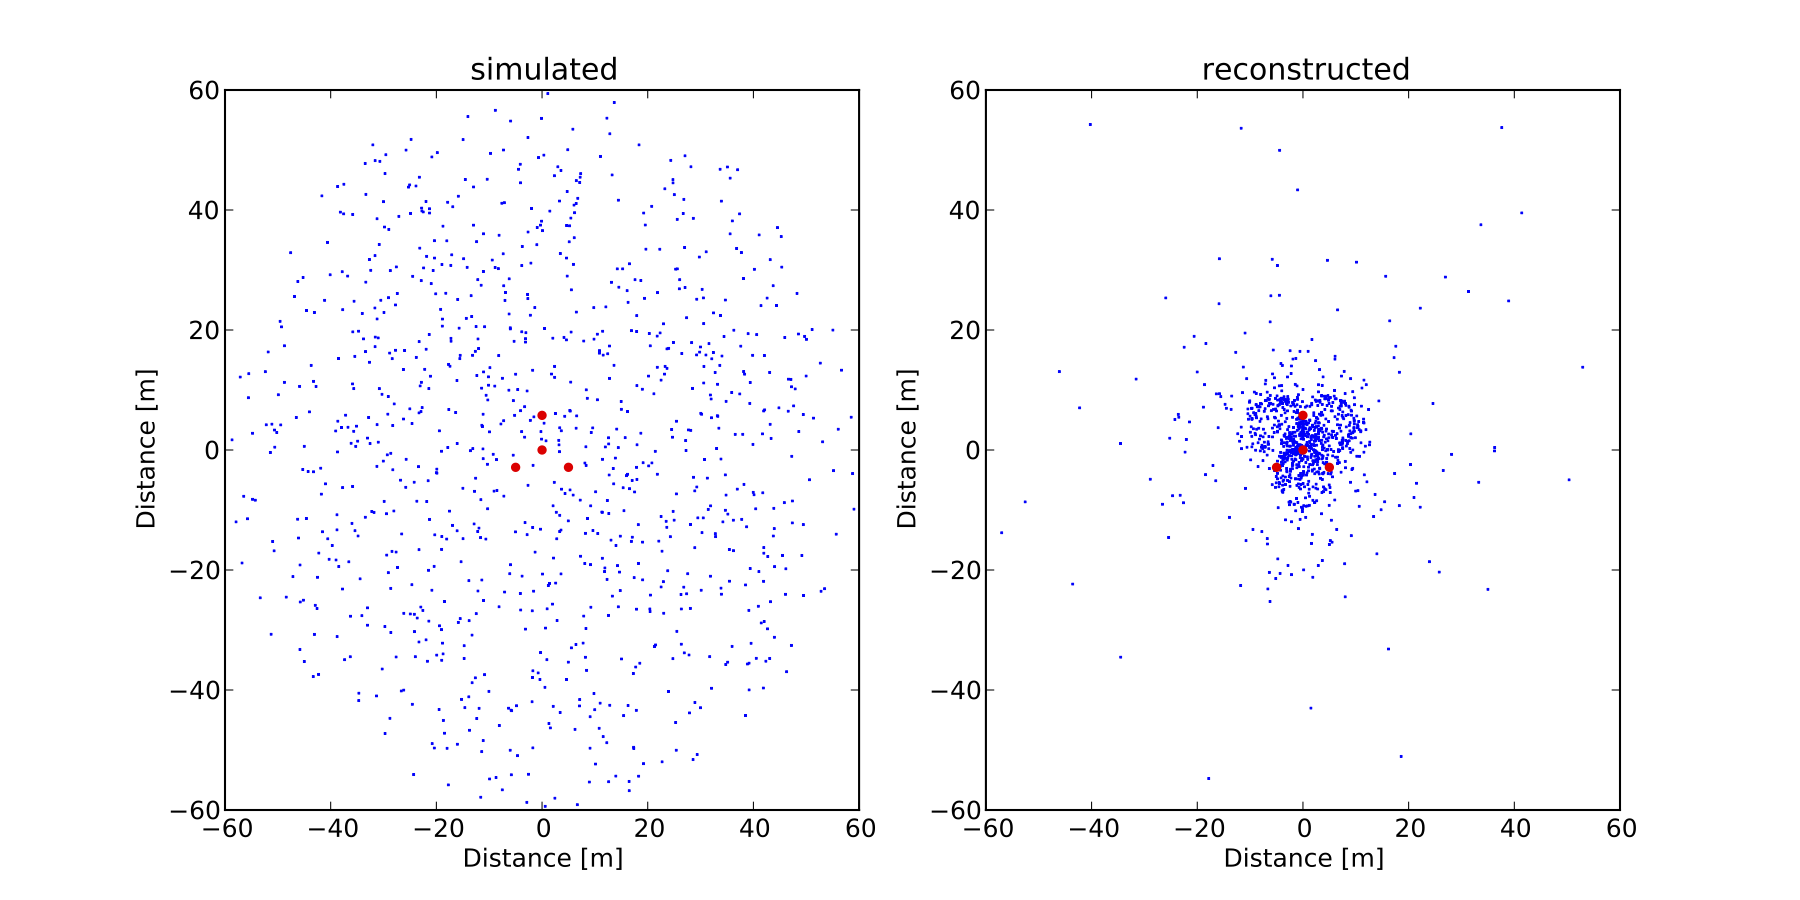
\includegraphics[width=.8\linewidth]{raw-plots/COR-plot_scatter_reconstructed_core-GROUND-GAUSS_20.png}
\caption{Simulated (left) and reconstructed (right) shower core positions for a
\SI{1}{\peta\electronvolt} vertical proton.
The detector signals have been simulated using the simulations
discussed in \chref{ch:reconstruction}.  The detectors no longer have
knowledge about the particle densities in the shower, but can only observe the
few particles that traverse the detectors.  This severely limits the
accuracy of the reconstruction of the core position.}
\label{fig:core-twob}
\end{figure}

Once the core position is determined, the full lateral distribution function
(\eqref{eq:ldf}) can be fitted to the approximate densities to obtain the shower
size.
\figref{fig:shower-size} shows the size of the shower obtained by analyzing
simulated detector signals.
The vertical showers have been created by protons with an energy of
\SI{1}{\peta\electronvolt}, equivalent to a shower size of $\lg N_e = 4.8$
particles. The shower size is underestimated for most events.
\begin{figure}
\centering
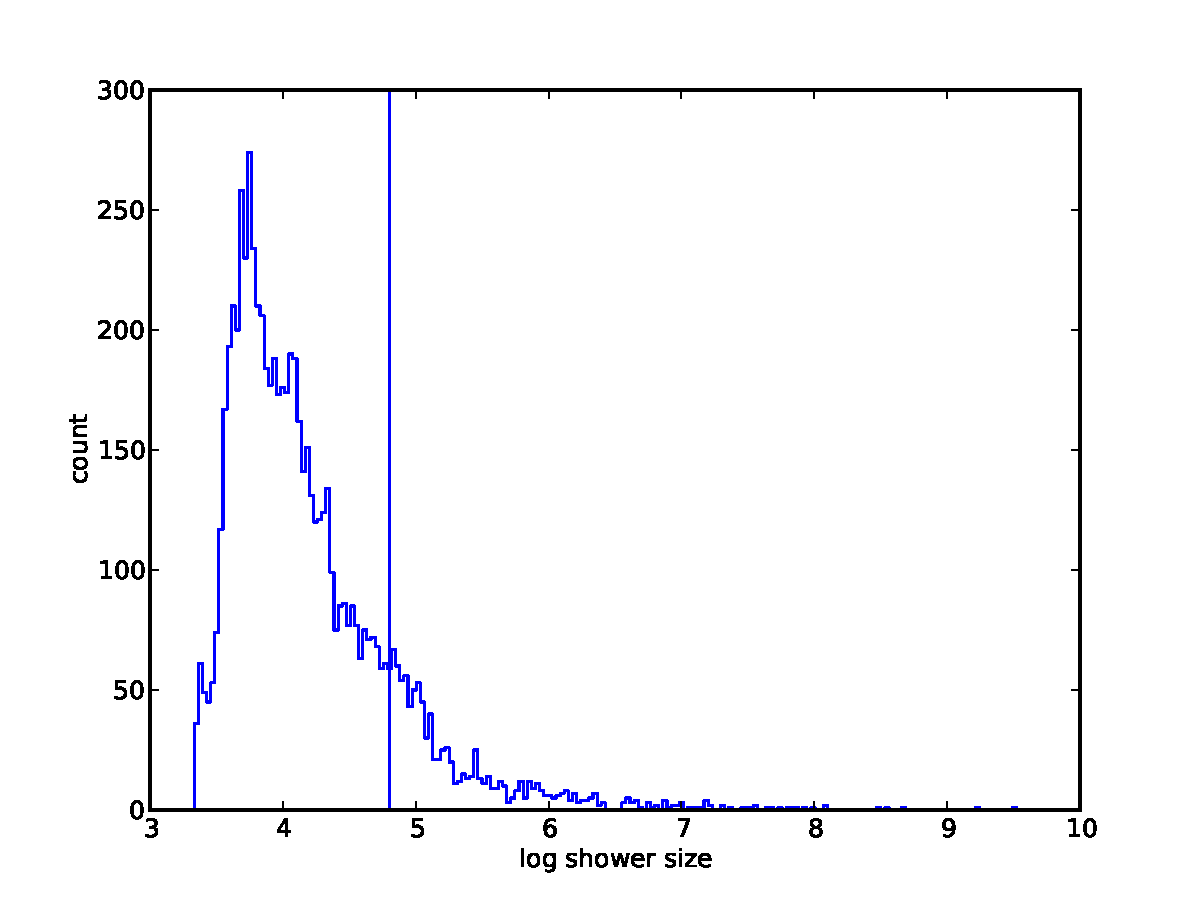
\includegraphics[width=.8\linewidth]{raw-plots/COR-plot_shower_size_hist-GROUND-GAUSS_20.pdf}
\caption{Reconstruction of shower size.  The vertical showers have been
created by protons with an energy of \SI{1}{\peta\electronvolt},
equivalent to a shower size of $\lg N_e$ = $4.8$ particles.  The shower size is
underestimated for most events.}
\label{fig:shower-size}
\end{figure}

Thorough investigations are required to make a rigorous treatment of the shower
size reconstruction. \textcite{Steijger:2012-energy} has suggested the use of
statistical tests to reject events which can not be accurately reconstructed.
Ongoing work by Bosboom will be published in \cite{Bosboom:2012}.
